\documentclass{article}
\usepackage[utf8]{inputenc}
\usepackage{fancyhdr}
\usepackage{graphicx}

% ---- Commands ------- %
\newcommand{\documentNumber}[1]{
    \LARGE  \textbf{ PUSP2142{#1} } \\
    \medskip
}
\newcommand{\documentVersion}[1]{
    v.{#1} \\
    \medskip
}
\newcommand{\documentTitle}[1]{
    \centerline{\rule{13cm}{0.4pt}}
    \bigskip \bigskip
    \LARGE {#1} \\
    \bigskip \bigskip
    \centerline{\rule{13cm}{0.4pt}}
}
\newcommand{\documentGroup}[1]{
    \bigskip \bigskip
    \LARGE Group {#1} \\
    \bigskip
}
\newcommand{\documentResponsible}[1]{
    \LARGE Responsible: {#1} \\
    \medskip
}
\newcommand{\documentAuthors}[1]{
    \LARGE Authors: {#1} \\
    \medskip    
}
\newcommand{\documentDate}[1]{
    \date {#1} 
}

\graphicspath{{./images/}} %Defines a path to file images

% --- Header & Footer ---- %
\pagestyle{fancy}
\lhead{\leftmark}
\rhead{}
\rfoot{\thepage}
\cfoot{}
\lfoot{}


% ------------------------------------------------ #

% ----- FILL THIS ----- %
\title {
    % Must be 2 digits
    \documentNumber {01}    
    
    \documentVersion {0.1}
    
    % Full name - SHORTNAME
    \documentTitle {Template}
    \documentGroup {2}
    
    % Options: - Project management Group
    %          - System architecture Group
    %          - Developer Group
    %          - Test Group
    \documentResponsible {Project management Group}
    \documentAuthors {Project management group}
    
    % Format: YYYY-MM-DD
    \documentDate {2021-01-25}
}

\begin{document}

\maketitle
\thispagestyle{empty}

\newpage

\tableofcontents

\newpage



\section{Introduction}

This document presents requirements for the (Sätt in namn). (Sätt in namn) is a system which purpose and main functionality is to administer time reporting with web-usage capabilities. 


\section{Reference documents}

\begin{enumerate}
  \item Software Requirements Specification: BaseBlockSystem, v. 1.0, Doc. number: PUSS12002
  \item The requirements on the usability of the system applies to this document and are therefore implemented in “System-namn”, following requirements are implemented; 6.1.1, 6.1.2, 6.1.3, 6.1.4, 6.1.6, 6.1.8, 6.1.9, 6.2.2
\end{enumerate}

\section{Background and goals}
\subsection{Main goals}

The goal is to develop and distribute a web-based system where the user can report time and administrate the system according to their roles.

\subsection{Actors and their objectives}
The system can be used and administrated by following actors;

\begin{itemize}
  \item \textbf{User:} The user has the authority to log in to the system to report and  change past reported time as well as review their reported times. The user also inherits roles as either "SG", "UG", and "TG".
  \item \textbf{Project Leader:}
  The project leaders main objective is to administer groups within the project, this implies that the project leader has the authority to add and remove as well as assign users from/to designated roles.
   \item \textbf{Administrator:} The administrator has the authority to add and remove users from the system along with creating and removing project groups. The admin is the only role that can assign the role “Project leader” to a user. The main goal of this role is to be able to administrate creation and removal of users.
\end{itemize}

\begin{figure}[placement specifier]
\centering
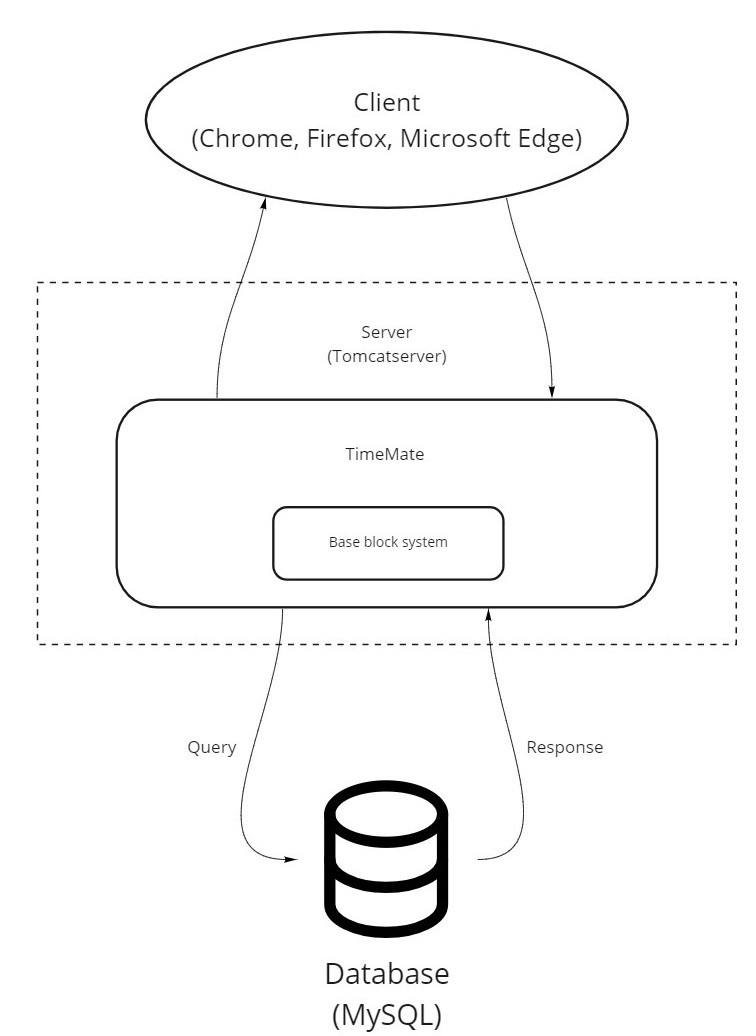
\includegraphics[width=0.5\textwidth]{Flowchart_6.jpg}
\caption{Context diagram}
\end{figure}

\caption{Image is to complex to understand}

\section{Terminology}



\section{Context diagram}

\section{Functional requirements}
\subsection{Login and logout}
\subsubsection{Requirement}
Scenario 6.1.3 should be supported by the system.

\subsubsection{Requirement}
 When  a  user  reaches  the  system  and  is  not  logged  in he/she should be asked to provide a username and a password.  No other information should be provided to the user.

\subsubsection{Requirement}
The user should not be able to change their passwords to their previous one.

\subsubsection{Requirement}
If the user has forgotten their password, they should be able to get a newly generated password from the server by email.

\subsubsection{Requirement}
New users should be assigned passwords generated by the server according to the password ruleset.

\subsubsection{Requirement}
Users should be able to change their password on the “My profile” page.
\subsubsection{Requirement}
Inputs of passwords not existing in the database should return an error message.
\subsubsection{Requirement }
Inputs of incorrect data (e.g. negative numbers or non-valid dates etc.) should return an error message.
\subsubsection{Requirement }
Usernames should be unique. Inputs of new users with existing names should return an error message.
\subsubsection{Requirement}
If the administrator tries to add a new user with a username that breaks the ruleset, an error message should be returned.
\subsubsection{Requirement}
Inputs of new passwords which are identical to the users previous password should return an error message. 
\subsubsection{Requirement}
Error messages should be in the following format: ”Error code – Reason”.


\begin{figure}[placement specifier]
\centering
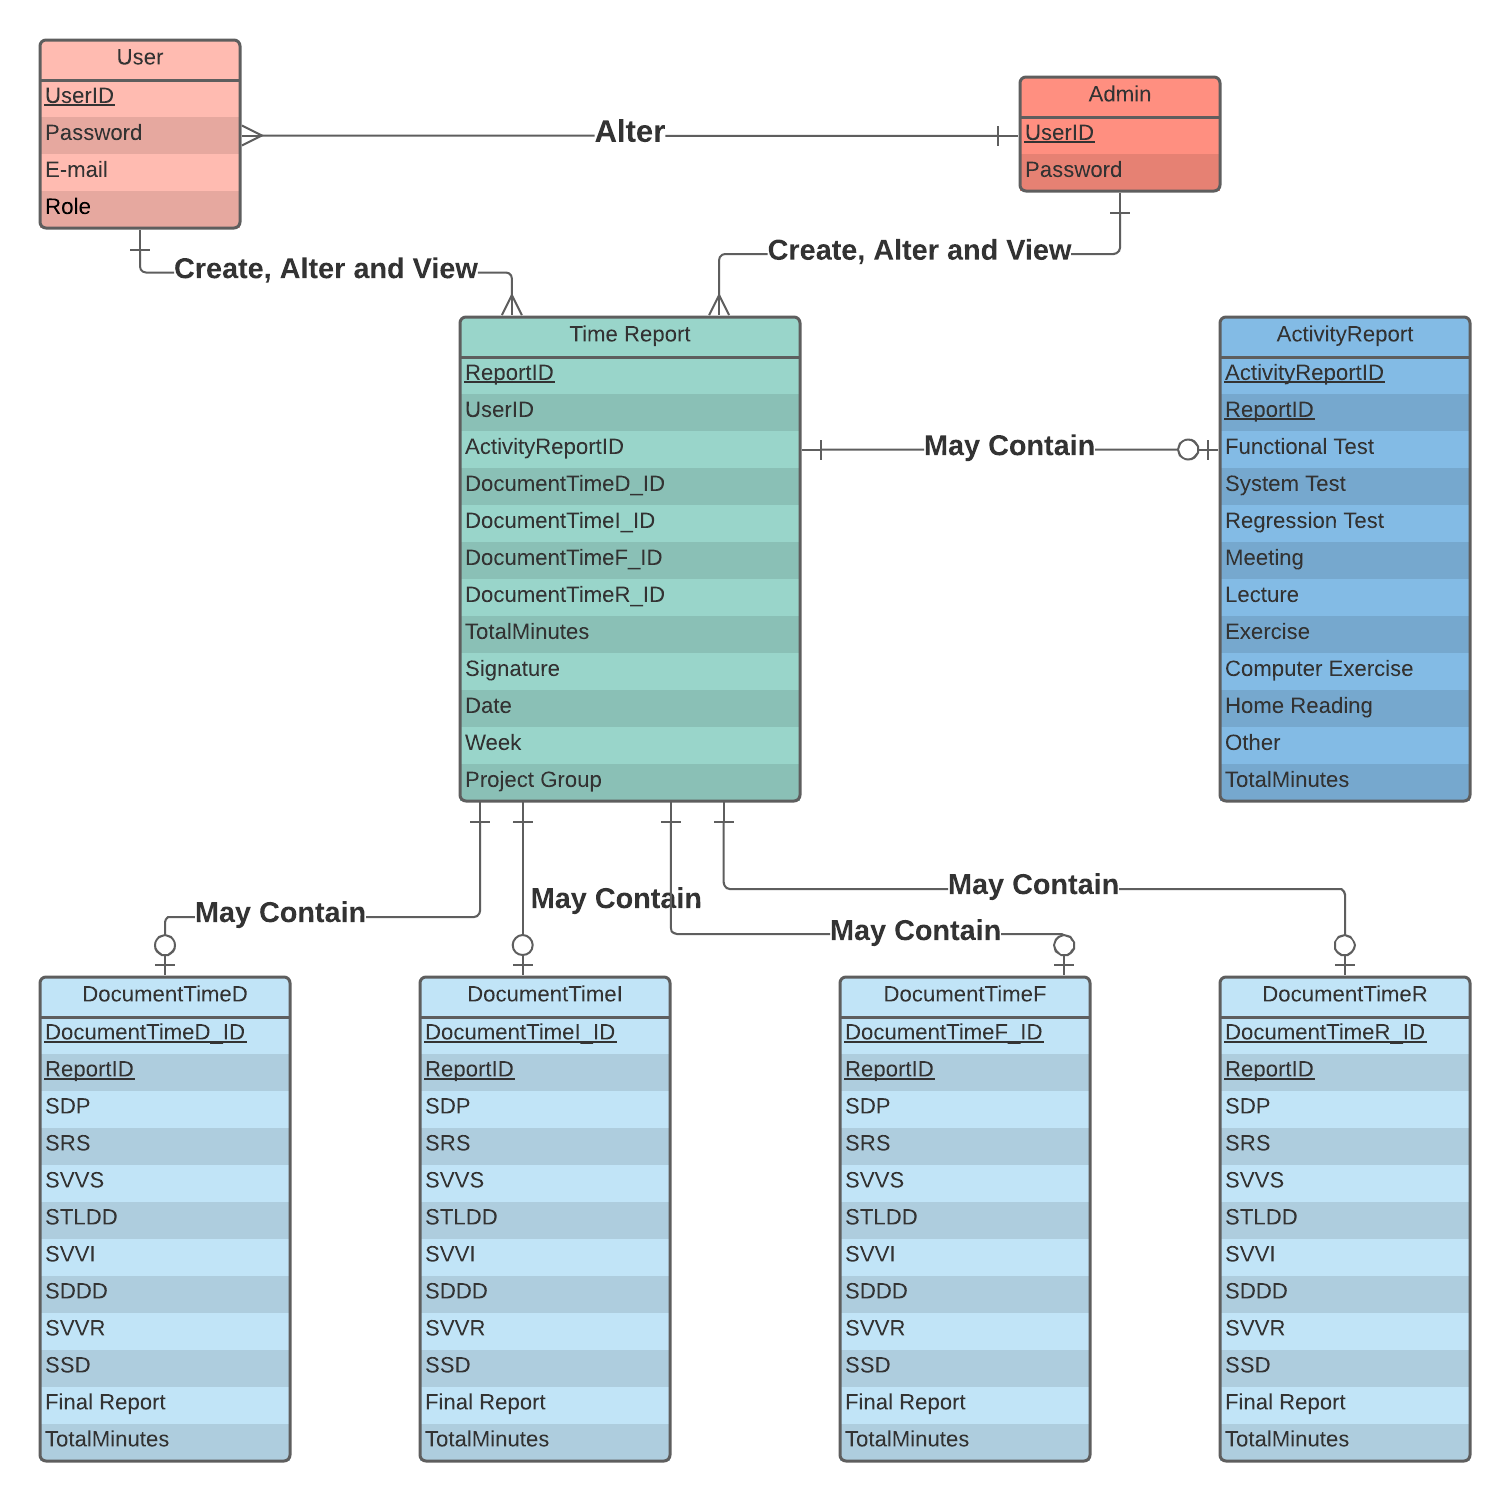
\includegraphics[width=0.5\textwidth]{PUSPERdiagram.png}
\caption{ER-diagram}
\end{figure}





\subsection{Data}
\subsubsection{Requirement}
A password should consist of at least one character of each type. [a-z][A-Z][1-9] with a minimum of 8 characters.
\subsubsection{Requirement (SÄTT NUMMER}
\subsubsection{Requirement (SÄTT NUMMER} 

\subsection{User}
\subsubsection{Requirement}
A user can create and submit a time report to the project group which they are assigned to.
\subsubsection{Requirement}
The following scenario should be supported by the system;

\textbf{Scenario:} The user wants to submit a time report

\textbf{Prerequisites} The user is logged in to the system

\begin{enumerate}


\item The user navigates to the page “Time Report”. 
\item The user is presented with an overview of their previously reported time. 
\item The user presses the button “Create New Time Report”
\item The user fills in the blank textboxes with the time they have spent on the different activities.
\item The user presses the button for “Submit”.
\item The user is presented with a popup window confirming that the changes have been made.
\item An updated view of the page is displayed.
\end{enumerate}

\subsubsection{Requirement 6.5.3}
A user should be able to see a summarized view of previous reported time.

\subsubsection{Requirement 6.5.4}
The following scenario should be supported by the system;\\

\textbf{Scenario:} The user wants to see a summary of their reported time.

\textbf{Prerequisites} The user is logged in to the system
\begin{enumerate}


\item The user navigates to the page “Time report”.
\item A page is displayed which includes the option to report time, edit old time reports but also a summarized view of their previously logged time. 
\end{enumerate}

\subsubsection{Requirement 6.5.5}
A user should be able to change their time report after it has been submitted to the system.
\subsubsection{Requirement 6.5.6}
A user should be able to delete a previously submitted time report.
\subsubsection{Requirement 6.5.7}
The following scenario should be supported by the system;\\

\textbf{Scenario:} A user wants to change or delete previously reported time.

\textbf{Prerequisites} The user is logged in to the system

\begin{enumerate}

\item The user navigates to the page “Time report”.
\item The user is presented with an overview of their previously reported time. 
\item The user presses the button “Edit time report”
\item The user chooses a time report.
\item The user is presented with a new page which includes the previously reported time table and a button for “Delete”. 
\item The user adds/fills in the new time or chooses to delete the report.
\item The user clicks on the button “Submit Change”.
\item The user is presented with a popup window confirming that the changes have been made.  
\item An updated view of the page is displayed.

\end{enumerate}
\subsubsection{Requirement}
A user should be able to change their password.
\subsubsection{Requirement}
A password should consist of at least one character of each type. [a-z][A-Z][1-9] with a minimum of 8 characters.

\subsubsection{Requirement}
The following scenario should be supported by the system;\\

\textbf{Scenario:} A user wants to change their password.

\textbf{Prerequisites} The user is logged in to the system

\begin{enumerate}
    \item The user clicks on the “Change Password” button in the menu.
    \item The user is presented with a page which includes three relevant textboxes.
    \item The user fills in the first textbox with their current password.
    \item The user fills in the second textbox with their new password.
    \item The user repeats their new password in the third textbox.
    \item The user clicks the button “Change Password”.
    \item The user's password is changed in the system.
    \item The user is presented with a popup window confirming that the changes has been made.
\end{enumerate}



\subsubsection{Requirement}
The following scenario should be supported by the system;

\textbf{Scenario:} A user wants to change their password with invalid entry.

\textbf{Prerequisites} The user is logged in to the system

\begin{enumerate}
    \item The user clicks on the “Change Password” button in the menu.
    \item The user is presented with a page which includes three relevant textboxes.
    \item The user fills in the first textbox with their current password.
    \item The user fills in the second textbox with their new password which does not meet requirement 6.2.1.
    \item The user repeats their new password in the third textbox.
    \item The user clicks the button “Change Password”.
    \item The user's password is not changed and a popup window with an error message is displayed.
    \item The user is sent back to stage 3.
\end{enumerate}

\subsection{Project Leader}
\subsubsection{Requirement}
The following scenario should be supported by the system.
\textbf{Scenario:} The project leader tries to acquire a summary of reported time.
\textbf{Prerequisites:} Time to be summarized exists, user has the role "Project leader" and the user is on the "Time Reporting" page.

\begin{enumerate}
    \item The project leader clicks on the administration page 
    \item The project leader clicks on the “SHOW SIGNED REPORTS” button.
    \item A list with user’s name and the total reported time will be displayed,
    \item The project leader clicks on a user name and it displays the user’s time reports.
\end{enumerate}
\subsubsection{Requirement}
The following scenario should be supported by the system.
\textbf{Scenario:} Project leader tries to sign a weekly report
\textbf{Prerequisites:} User has the role ”Project leader”, weekly reports exist, and the user has clicked on the “Sign Time Reports” button.

\begin{enumerate}
    \item A list of all the unsigned weekly reports is shown to the project leader.
    \item The project leader can sign the reports by clicking on the corresponding checkbox.
    \item The project leader confirms their selection by pressing on the “Confirm” button
    \item The system sends the changes to the server.
    \item The system returns an updated list of unsigned reports, or an empty list if none exists
\end{enumerate}
\subsubsection{Requirement}

\subsection{Administrator}
\subsubsection{Requirement}
The following scenario should be supported by the system.

\textbf{Scenario:} The administrator tries to add a user.

\textbf{Prerequisites:} The administrator is on the “Administration” page

\begin{enumerate}
    \item The administrator clicks on the button to add a user.
    \item The administrator inputs the name of the user.
    \item The inputs are sent to the server which adds it to the database and generates a password.
    \item The system creates a new entry in the user list and inserts the inputted name.
    \item The server returns the password to the corresponding field in the user list.
    \item The user clicks the button “Change Password”.
    \item The updated user list is shown to the administrator.
\end{enumerate}

\subsubsection{Requirement}
The following scenario should be supported by the system.

\textbf{Scenario:} The Administrator tries to add a user with the same name.

\textbf{Prerequisites:} The administrator is on the “Administration” page

\begin{enumerate}
    \item The administrator clicks on the button to add a user.
    \item The administrator inputs the name of the user.
    \item The inputs are sent to the server, which notices that the name already exists in the database.
    \item The server does not accept the inputted name.
    \item The admin is told that the user already exists with a message.
\end{enumerate}

\subsubsection{Requirement}
The following scenario should be supported by the system.

\textbf{Scenario:} The administrator tries to remove a user.

\textbf{Prerequisites:} The administrator is on the “Administration” page

\begin{enumerate}
    \item The Administrator clicks on the button to remove the user.
    \item The Administrator must confirm the removal by typing in the user’s name and click on the “confirm” button.
    \item The information is sent to the server.
    \item The user is removed from the database.
    \item The page is updated with the new user list, with a message confirming the change.
\end{enumerate}

\subsubsection{Requirement}
The following scenario should be supported by the system.

\textbf{Scenario:} The administrator tries to assign a role to a user.

\textbf{Prerequisites:} The administrator is on the “Management” page

\begin{enumerate}
    \item Administrator clicks on the user management page.
    \item Administrator chooses the user’s group role.
    \item Administrator should verify it by clicking the “CONFIRM” button.
    \item User’s role is added.
    \item Information is sent to the server.
\end{enumerate}

\subsubsection{Requirement}
The following scenario should be supported by the system.

\textbf{Scenario:} The administrator tries to assign a role to a user.

\textbf{Prerequisites:} The administrator is on the “Management” page

\begin{enumerate}
    \item Administrator clicks on the user management page.
    \item Administrator chooses the user’s group role.
    \item Administrator should verify it by clicking the “CONFIRM” button.
    \item User’s role is added.
    \item Information is sent to the server.
\end{enumerate}

\subsubsection{Requirement}
All users in the database should be shown as a list on the “Administration” page.

\subsubsection{Requirement}
The following scenario should be supported by the system.
\textbf{Scenario:} The administrator tries to acquire a summary of reported time.
\textbf{Prerequisites:} Time to be summarized exists.

\begin{enumerate}
    \item The administrator clicks on the administration page 
    \item The administrator clicks on the “SHOW SIGNED REPORTS” button.
    \item A list with user’s name and the total reported time will be displayed,
    \item The admin clicks on a user name and it displays the user’s time reports.
\end{enumerate}

\subsubsection{Requirement}
The following scenario should be supported by the system.

\textbf{Scenario:} The administrator tries to assign a role to a user.

\textbf{Prerequisites:} The administrator is on the administration page.

\begin{enumerate}
    \item The admin clicks on “view”.
    \item A list with all users and their roles is displayed.
    \item The administrator clicks on the role-alternative.
    \item The admin can change the role of the user by clicking on a new role and confirming it.
    \item The information is saved and sent to the server
    \item The database is updated with the changes.
\end{enumerate}



\section{Quality Requirements}
\subsection{Maintainability}
\subsubsection{Requirement}
See requirement 7.1.1 in PUSS12002.
\subsection{Performance}
\subsubsection{Requirement}
See requirement 7.2.1 in PUSS12002.




\section{Project requirements}
\subsection{Development environment}
\subsubsection{Requirement 9.1}
The back end for the system should use Java JDK 11 as development environment.

\subsubsection{Requirement 9.2}
The front end for the system should use Bootstrap v.4.5.3.

\subsubsection{Requirement 9.3}
The database should be developed in MySQL.

\end{document}
